%%
%% Meta: Boxplot erstellen. Viele Beispiele
%%

\input{bbwLayoutPage}

\renewcommand{\metaHeaderLine}{Arbeitsblatt}
\renewcommand{\arbeitsblattTitel}{Boxplot}

%%%%%%%%%%%%%%%%%%%%%%%%%%%%%%%%%%%%%%%%%%%%%%%%%%%%%%%%%%%%%%%%%%

%\usepackage{amssymb} 
\usepackage{cancel}

\newcommand\Ccancel[2][black]{\renewcommand\CancelColor{\color{#1}}\cancel{#2}}


\begin{document}%%
\arbeitsblattHeader{}
\section{Boxplot}
Erstellen Sie Boxplots...

\TRAINER{Trainer-Version (Lösungen ganz unten.)}

\begin{itemize}
\item Finden Sie zunächst jeweils den Median und die beiden Quartile
(M, Q1, Q3).
\item Geben Sie die Skala an (dafür ist jeweils eine Linie
vorgesehen).
\item Zeichnen Sie Median und die beiden Quartile ein und schließen
Sie die Box.
\item Berechnen Sie IQR (Interquartilsrange) $\textrm{IQR} = \textrm{Q3} - \textrm{Q1}$
\item Berechnen Sie den 1.5fachen Interquartilsabstand
($1.5\cdot{}(\textrm{Q3}-\textrm{Q1}) = 1.5 \cdot \textrm{IRQ}$).
\item Zeichnen Sie fein (so dass Sie es wieder ausradieren können) die beiden
Ausreißerschwellen ein. Diese liegt beim 1.5fachen Quartilsabstand
unter bzw über der Box.
\item Zeichnen Sie die Whisker\footnote{Erinnert an Whiskas?}
(Antennen, Fühler) und  allfällige Ausreißer als kleine Ringe ein.
\end{itemize}

\newcommand{\boxplot}[2]{
\subsection{Daten}
\begin{tabular}{#1}
\hline
#2\\
\hline
\end{tabular}

\subsubsection*{Boxplot}
\noTRAINER{\mmPapier{1.6}}
}%% end definition "BOXPLOT"


\boxplot{|c|c|c|c|c|c|c|}{7&8&8&9&11&15&21}

\boxplot{|c|c|c|c|c|c|c|c|}{7&8&8&9&9&11&15&21}

\newpage
\boxplot{|c|c|c|c|c|c|c|c|c|}{1&7&8&8&9&9&11&15&25}

\boxplot{|c|c|c|c|c|c|c|c|c|c|}{7&8&8&9&9&11&15&21&22&45}

\boxplot{|c|c|c|c|c|c|c|c|c|c|c|}{23&50&95&96&98&101&102&106&106&112&150}

\section{Interpretation}
Interpretieren Sie den folgenden Boxplot.
\begin{center}
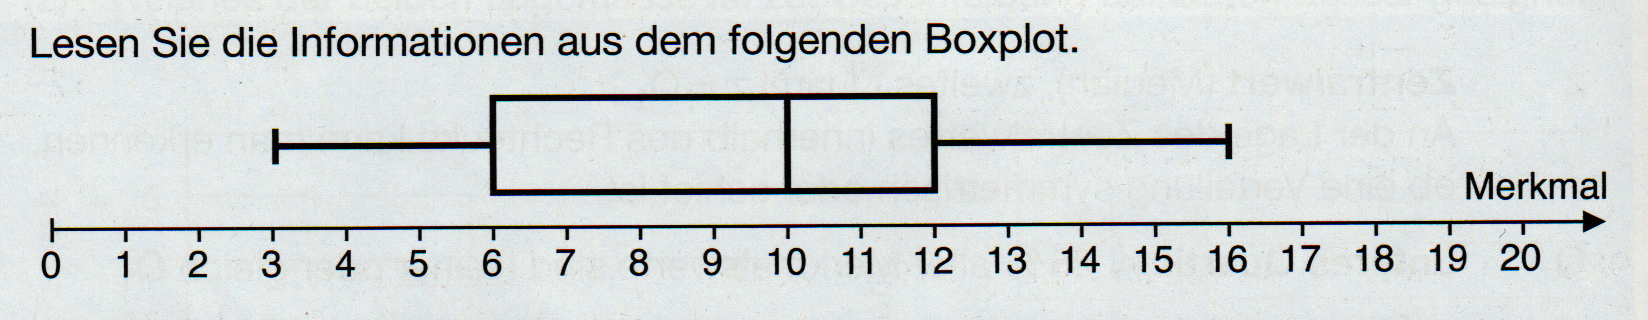
\includegraphics[width=15cm]{img/BoxplotAufgabeFrommenwiler.png}
\end{center}
\TRAINER{Lösungen
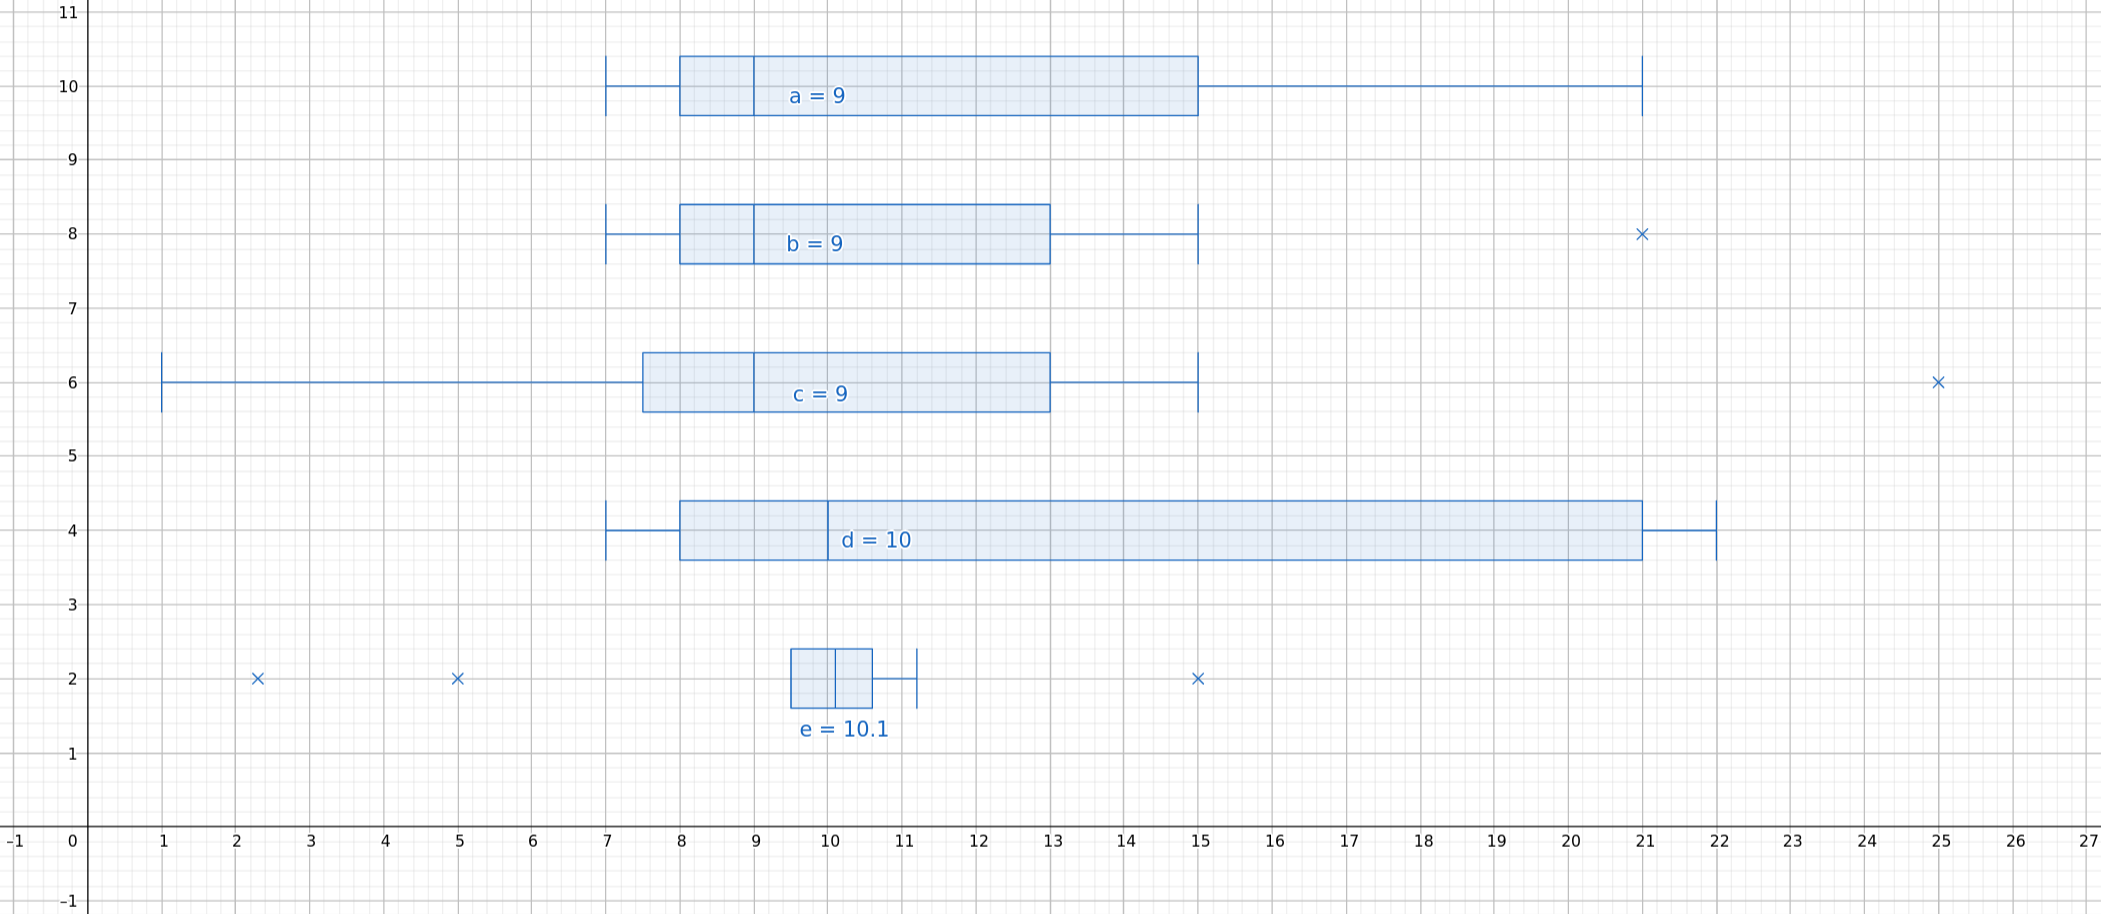
\includegraphics[width=15cm]{img/Loesungen.png}
}
\end{document}
